
%% bare_conf.tex
%% V1.3
%% 2007/01/11
%% by Michael Shell
%% See:
%% http://www.michaelshell.org/
%% for current contact information.
%%
%% This is a skeleton file demonstrating the use of IEEEtran.cls
%% (requires IEEEtran.cls version 1.7 or later) with an IEEE conference paper.
%%
%% Support sites:
%% http://www.michaelshell.org/tex/ieeetran/
%% http://www.ctan.org/tex-archive/macros/latex/contrib/IEEEtran/
%% and
%% http://www.ieee.org/

%%*************************************************************************
%% Legal Notice:
%% This code is offered as-is without any warranty either expressed or
%% implied; without even the implied warranty of MERCHANTABILITY or
%% FITNESS FOR A PARTICULAR PURPOSE! 
%% User assumes all risk.
%% In no event shall IEEE or any contributor to this code be liable for
%% any damages or losses, including, but not limited to, incidental,
%% consequential, or any other damages, resulting from the use or misuse
%% of any information contained here.
%%
%% All comments are the opinions of their respective authors and are not
%% necessarily endorsed by the IEEE.
%%
%% This work is distributed under the LaTeX Project Public License (LPPL)
%% ( http://www.latex-project.org/ ) version 1.3, and may be freely used,
%% distributed and modified. A copy of the LPPL, version 1.3, is included
%% in the base LaTeX documentation of all distributions of LaTeX released
%% 2003/12/01 or later.
%% Retain all contribution notices and credits.
%% ** Modified files should be clearly indicated as such, including  **
%% ** renaming them and changing author support contact information. **
%%
%% File list of work: IEEEtran.cls, IEEEtran_HOWTO.pdf, bare_adv.tex,
%%                    bare_conf.tex, bare_jrnl.tex, bare_jrnl_compsoc.tex
%%*************************************************************************

% *** Authors should verify (and, if needed, correct) their LaTeX system  ***
% *** with the testflow diagnostic prior to trusting their LaTeX platform ***
% *** with production work. IEEE's font choices can trigger bugs that do  ***
% *** not appear when using other class files.                            ***
% The testflow support page is at:
% http://www.michaelshell.org/tex/testflow/



% Note that the a4paper option is mainly intended so that authors in
% countries using A4 can easily print to A4 and see how their papers will
% look in print - the typesetting of the document will not typically be
% affected with changes in paper size (but the bottom and side margins will).
% Use the testflow package mentioned above to verify correct handling of
% both paper sizes by the user's LaTeX system.
%
% Also note that the "draftcls" or "draftclsnofoot", not "draft", option
% should be used if it is desired that the figures are to be displayed in
% draft mode.
%
\documentclass[conference]{IEEEtran}
% Add the compsoc option for Computer Society conferences.
%
% If IEEEtran.cls has not been installed into the LaTeX system files,
% manually specify the path to it like:
% \documentclass[conference]{../sty/IEEEtran}





% Some very useful LaTeX packages include:
% (uncomment the ones you want to load)


% *** MISC UTILITY PACKAGES ***
%
%\usepackage{ifpdf}
% Heiko Oberdiek's ifpdf.sty is very useful if you need conditional
% compilation based on whether the output is pdf or dvi.
% usage:
% \ifpdf
%   % pdf code
% \else
%   % dvi code
% \fi
% The latest version of ifpdf.sty can be obtained from:
% http://www.ctan.org/tex-archive/macros/latex/contrib/oberdiek/
% Also, note that IEEEtran.cls V1.7 and later provides a builtin
% \ifCLASSINFOpdf conditional that works the same way.
% When switching from latex to pdflatex and vice-versa, the compiler may
% have to be run twice to clear warning/error messages.






% *** CITATION PACKAGES ***
%
%\usepackage{cite}
% cite.sty was written by Donald Arseneau
% V1.6 and later of IEEEtran pre-defines the format of the cite.sty package
% \cite{} output to follow that of IEEE. Loading the cite package will
% result in citation numbers being automatically sorted and properly
% "compressed/ranged". e.g., [1], [9], [2], [7], [5], [6] without using
% cite.sty will become [1], [2], [5]--[7], [9] using cite.sty. cite.sty's
% \cite will automatically add leading space, if needed. Use cite.sty's
% noadjust option (cite.sty V3.8 and later) if you want to turn this off.
% cite.sty is already installed on most LaTeX systems. Be sure and use
% version 4.0 (2003-05-27) and later if using hyperref.sty. cite.sty does
% not currently provide for hyperlinked citations.
% The latest version can be obtained at:
% http://www.ctan.org/tex-archive/macros/latex/contrib/cite/
% The documentation is contained in the cite.sty file itself.






% *** GRAPHICS RELATED PACKAGES ***
%
\ifCLASSINFOpdf
\usepackage[pdftex]{graphicx}
  % declare the path(s) where your graphic files are
  % \graphicspath{{../pdf/}{../jpeg/}}
  % and their extensions so you won't have to specify these with
  % every instance of \includegraphics
  % \DeclareGraphicsExtensions{.pdf,.jpeg,.png}
\else
  % or other class option (dvipsone, dvipdf, if not using dvips). graphicx
  % will default to the driver specified in the system graphics.cfg if no
  % driver is specified.
  % \usepackage[dvips]{graphicx}
  % declare the path(s) where your graphic files are
  % \graphicspath{{../eps/}}
  % and their extensions so you won't have to specify these with
  % every instance of \includegraphics
  % \DeclareGraphicsExtensions{.eps}
\fi
% graphicx was written by David Carlisle and Sebastian Rahtz. It is
% required if you want graphics, photos, etc. graphicx.sty is already
% installed on most LaTeX systems. The latest version and documentation can
% be obtained at: 
% http://www.ctan.org/tex-archive/macros/latex/required/graphics/
% Another good source of documentation is "Using Imported Graphics in
% LaTeX2e" by Keith Reckdahl which can be found as epslatex.ps or
% epslatex.pdf at: http://www.ctan.org/tex-archive/info/
%
% latex, and pdflatex in dvi mode, support graphics in encapsulated
% postscript (.eps) format. pdflatex in pdf mode supports graphics
% in .pdf, .jpeg, .png and .mps (metapost) formats. Users should ensure
% that all non-photo figures use a vector format (.eps, .pdf, .mps) and
% not a bitmapped formats (.jpeg, .png). IEEE frowns on bitmapped formats
% which can result in "jaggedy"/blurry rendering of lines and letters as
% well as large increases in file sizes.
%
% You can find documentation about the pdfTeX application at:
% http://www.tug.org/applications/pdftex





% *** MATH PACKAGES ***
%
\usepackage[cmex10]{amsmath}
% A popular package from the American Mathematical Society that provides
% many useful and powerful commands for dealing with mathematics. If using
% it, be sure to load this package with the cmex10 option to ensure that
% only type 1 fonts will utilized at all point sizes. Without this option,
% it is possible that some math symbols, particularly those within
% footnotes, will be rendered in bitmap form which will result in a
% document that can not be IEEE Xplore compliant!
%
% Also, note that the amsmath package sets \interdisplaylinepenalty to 10000
% thus preventing page breaks from occurring within multiline equations. Use:
%\interdisplaylinepenalty=2500
% after loading amsmath to restore such page breaks as IEEEtran.cls normally
% does. amsmath.sty is already installed on most LaTeX systems. The latest
% version and documentation can be obtained at:
% http://www.ctan.org/tex-archive/macros/latex/required/amslatex/math/





% *** SPECIALIZED LIST PACKAGES ***
%
\usepackage{algorithmic}
% algorithmic.sty was written by Peter Williams and Rogerio Brito.
% This package provides an algorithmic environment fo describing algorithms.
% You can use the algorithmic environment in-text or within a figure
% environment to provide for a floating algorithm. Do NOT use the algorithm
% floating environment provided by algorithm.sty (by the same authors) or
% algorithm2e.sty (by Christophe Fiorio) as IEEE does not use dedicated
% algorithm float types and packages that provide these will not provide
% correct IEEE style captions. The latest version and documentation of
% algorithmic.sty can be obtained at:
% http://www.ctan.org/tex-archive/macros/latex/contrib/algorithms/
% There is also a support site at:
% http://algorithms.berlios.de/index.html
% Also of interest may be the (relatively newer and more customizable)
% algorithmicx.sty package by Szasz Janos:
% http://www.ctan.org/tex-archive/macros/latex/contrib/algorithmicx/




% *** ALIGNMENT PACKAGES ***
%
%\usepackage{array}
% Frank Mittelbach's and David Carlisle's array.sty patches and improves
% the standard LaTeX2e array and tabular environments to provide better
% appearance and additional user controls. As the default LaTeX2e table
% generation code is lacking to the point of almost being broken with
% respect to the quality of the end results, all users are strongly
% advised to use an enhanced (at the very least that provided by array.sty)
% set of table tools. array.sty is already installed on most systems. The
% latest version and documentation can be obtained at:
% http://www.ctan.org/tex-archive/macros/latex/required/tools/


\usepackage{mdwmath}
\usepackage{mdwtab}
% Also highly recommended is Mark Wooding's extremely powerful MDW tools,
% especially mdwmath.sty and mdwtab.sty which are used to format equations
% and tables, respectively. The MDWtools set is already installed on most
% LaTeX systems. The lastest version and documentation is available at:
% http://www.ctan.org/tex-archive/macros/latex/contrib/mdwtools/


% IEEEtran contains the IEEEeqnarray family of commands that can be used to
% generate multiline equations as well as matrices, tables, etc., of high
% quality.


%\usepackage{eqparbox}
% Also of notable interest is Scott Pakin's eqparbox package for creating
% (automatically sized) equal width boxes - aka "natural width parboxes".
% Available at:
% http://www.ctan.org/tex-archive/macros/latex/contrib/eqparbox/





% *** SUBFIGURE PACKAGES ***
%\usepackage[tight,footnotesize]{subfigure}
% subfigure.sty was written by Steven Douglas Cochran. This package makes it
% easy to put subfigures in your figures. e.g., "Figure 1a and 1b". For IEEE
% work, it is a good idea to load it with the tight package option to reduce
% the amount of white space around the subfigures. subfigure.sty is already
% installed on most LaTeX systems. The latest version and documentation can
% be obtained at:
% http://www.ctan.org/tex-archive/obsolete/macros/latex/contrib/subfigure/
% subfigure.sty has been superceeded by subfig.sty.



%\usepackage[caption=false]{caption}
%\usepackage[font=footnotesize]{subfig}
% subfig.sty, also written by Steven Douglas Cochran, is the modern
% replacement for subfigure.sty. However, subfig.sty requires and
% automatically loads Axel Sommerfeldt's caption.sty which will override
% IEEEtran.cls handling of captions and this will result in nonIEEE style
% figure/table captions. To prevent this problem, be sure and preload
% caption.sty with its "caption=false" package option. This is will preserve
% IEEEtran.cls handing of captions. Version 1.3 (2005/06/28) and later 
% (recommended due to many improvements over 1.2) of subfig.sty supports
% the caption=false option directly:
%\usepackage[caption=false,font=footnotesize]{subfig}
%
% The latest version and documentation can be obtained at:
% http://www.ctan.org/tex-archive/macros/latex/contrib/subfig/
% The latest version and documentation of caption.sty can be obtained at:
% http://www.ctan.org/tex-archive/macros/latex/contrib/caption/




% *** FLOAT PACKAGES ***
%
%\usepackage{fixltx2e}
% fixltx2e, the successor to the earlier fix2col.sty, was written by
% Frank Mittelbach and David Carlisle. This package corrects a few problems
% in the LaTeX2e kernel, the most notable of which is that in current
% LaTeX2e releases, the ordering of single and double column floats is not
% guaranteed to be preserved. Thus, an unpatched LaTeX2e can allow a
% single column figure to be placed prior to an earlier double column
% figure. The latest version and documentation can be found at:
% http://www.ctan.org/tex-archive/macros/latex/base/



%\usepackage{stfloats}
% stfloats.sty was written by Sigitas Tolusis. This package gives LaTeX2e
% the ability to do double column floats at the bottom of the page as well
% as the top. (e.g., "\begin{figure*}[!b]" is not normally possible in
% LaTeX2e). It also provides a command:
%\fnbelowfloat
% to enable the placement of footnotes below bottom floats (the standard
% LaTeX2e kernel puts them above bottom floats). This is an invasive package
% which rewrites many portions of the LaTeX2e float routines. It may not work
% with other packages that modify the LaTeX2e float routines. The latest
% version and documentation can be obtained at:
% http://www.ctan.org/tex-archive/macros/latex/contrib/sttools/
% Documentation is contained in the stfloats.sty comments as well as in the
% presfull.pdf file. Do not use the stfloats baselinefloat ability as IEEE
% does not allow \baselineskip to stretch. Authors submitting work to the
% IEEE should note that IEEE rarely uses double column equations and
% that authors should try to avoid such use. Do not be tempted to use the
% cuted.sty or midfloat.sty packages (also by Sigitas Tolusis) as IEEE does
% not format its papers in such ways.





% *** PDF, URL AND HYPERLINK PACKAGES ***
%
%\usepackage{url}
% url.sty was written by Donald Arseneau. It provides better support for
% handling and breaking URLs. url.sty is already installed on most LaTeX
% systems. The latest version can be obtained at:
% http://www.ctan.org/tex-archive/macros/latex/contrib/misc/
% Read the url.sty source comments for usage information. Basically,
% \url{my_url_here}.





% *** Do not adjust lengths that control margins, column widths, etc. ***
% *** Do not use packages that alter fonts (such as pslatex).         ***
% There should be no need to do such things with IEEEtran.cls V1.6 and later.
% (Unless specifically asked to do so by the journal or conference you plan
% to submit to, of course. )

\begin{document}
%
% paper title
% can use linebreaks \\ within to get better formatting as desired
\title{What happens in Vegas: Analysis of Web Crawl data for context of a location}


% author names and affiliations
% use a multiple column layout for up to three different
% affiliations
\author{\IEEEauthorblockN{Primal Pappachan, Vikas Bansal, Abhishek Sethi}
\IEEEauthorblockA{Department of Computer Science and\\Electrical Engineering\\
University of Maryland Baltimore County\\
Baltimore, Maryland 21250 \\
primal1@umbc.edu, vikas1@umbc.edu, abse1@umbc.edu}}

% conference papers do not typically use \thanks and this command
% is locked out in conference mode. If really needed, such as for
% the acknowledgment of grants, issue a \IEEEoverridecommandlockouts
% after \documentclass

% for over three affiliations, or if they all won't fit within the width
% of the page, use this alternative format:
% 
%\author{\IEEEauthorblockN{Michael Shell\IEEEauthorrefmark{1},
%Homer Simpson\IEEEauthorrefmark{2},
%James Kirk\IEEEauthorrefmark{3}, 
%Montgomery Scott\IEEEauthorrefmark{3} and
%Eldon Tyrell\IEEEauthorrefmark{4}}
%\IEEEauthorblockA{\IEEEauthorrefmark{1}School of Electrical and Computer Engineering\\
%Georgia Institute of Technology,
%Atlanta, Georgia 30332--0250\\ Email: see http://www.michaelshell.org/contact.html}
%\IEEEauthorblockA{\IEEEauthorrefmark{2}Twentieth Century Fox, Springfield, USA\\
%Email: homer@thesimpsons.com}
%\IEEEauthorblockA{\IEEEauthorrefmark{3}Starfleet Academy, San Francisco, California 96678-2391\\
%Telephone: (800) 555--1212, Fax: (888) 555--1212}
%\IEEEauthorblockA{\IEEEauthorrefmark{4}Tyrell Inc., 123 Replicant Street, Los Angeles, California 90210--4321}}




% use for special paper notices
%\IEEEspecialpapernotice{(Invited Paper)}




% make the title area
\maketitle


\begin{abstract}
%\boldmath

Centipede is a web service which presents information about the context of a location from analysis of web crawl data. We have broadly defined context as belonging to one of the four categories: health, employment, weather and crime and also built a dictionary of these category related terms. By using Mapreduce we processed the data and stored it in MongoDB and visualized the results via a REST api. We also evaluated the results from centipede against Wikipedia and calculated precision, recall and F1 score. Results show that information learned by centipede matches closely with Wikipedia upto half of the time (50\%) and shows diverse results other times.     

\end{abstract}
% IEEEtran.cls defaults to using nonbold math in the Abstract.
% This preserves the distinction between vectors and scalars. However,
% if the conference you are submitting to favors bold math in the abstract,
% then you can use LaTeX's standard command \boldmath at the very start
% of the abstract to achieve this. Many IEEE journals/conferences frown on
% math in the abstract anyway.

% no keywords




% For peer review papers, you can put extra information on the cover
% page as needed:
% \ifCLASSOPTIONpeerreview
% \begin{center} \bfseries EDICS Category: 3-BBND \end{center}
% \fi
%
% For peerreview papers, this IEEEtran command inserts a page break and
% creates the second title. It will be ignored for other modes.
\IEEEpeerreviewmaketitle



\section{Introduction}
% no \IEEEPARstart
The need to search for sentiments on an entity has increased since the rapid growth of the Internet. An entity is defined to essentially be a noun, encapsulating people, places, and other things. People search for different entities in order to discover information on them, including what is the general view on that entity. This need to search for general views on different entities was the driving motivation behind the Centipede project. The goal of the Centipede project is to give users the ability to discover general attitudes towards specific entities. Though users can always perform multiple Google searches to uncover the information they need, the Centipede project removes the need to unnecessarily search through hundreds and possibly thousands of web pages. \\

The Centipede project takes web crawled data from the entire internet, and analyzes the web pages for general sentiments for different entities. The goal of the project is to provide the user with visually pleasing presentations of the general feelings towards an entity. Since there are billions of data sources, and an equal amount of entities, the primary entity used in this project was places. Places were essentially cities or different locations around the world. For locations, users commonly search for locations in order to discover the general feel for the location. Users want to know if the location is safe, is the weather nice, what kind of events are going on, how is the job market, etc. Centipede provides the user with different contexts to help the user answer such questions. For the purposes of Centipede, the contexts are defined as general categories of information that pertain to a specific location. 

The contexts defined for centipede are health, crime, employment, and weather. These contexts will contain information about how often each context is being discussed. For example, a question that Centipede could answer is how often employment is being discussed; answering the question about what is the employment status in a specific location like. Giving the user information about these different contexts provides the user enough information to make informed decisions about any location they desire without the need to scour across the web in search of articles discussing each context for a location. 


\subsection{Users}
The potential users of our service are travelers – people who want to know about trends in a place before traveling there, policy makers - who wants to evaluate the effect of public policies and rules and social response to them.
 
Anyone who is interested in a quick look and comparison of city context can also benefit from our service. In addition to helping people directly, output of our service can be used by several location based services which can enrich the experience of a smart phone user.

\subsection{Scenarios}

Suppose there is person who is travelling to Baltimore and staying there for a few days. Using our service, the person can identify various current trends in Baltimore and can participate in events according to his/her preference. 

Students can use our service before for selecting a university for higher studies based on trends in its location. S/he can get the trend information about crime, employment or weather before enrolling at the university. 

\section{Related Work}

While it is possible to read about a location from Wikipedia or Google News, these services are not very suited for finding categorized context of a location. The breadth of information provided by centipede is significantly larger than previously mentioned sources as it uses web crawl data for analysis. Unlike Wikipedia, this information automatically stays upto date and doesn't depend on users. On the other hand, media conglomerates might provide biased information to the users as it has been previously exposed \cite{med:one} \cite{med:two}.   

Previous work on analyzing web crawl data by \cite{semsim:lushan} has focused on building Semantic Textual Similarity Systems by analyzing web crawl data. Web crawl data has been used for building web indexes based on Page Rank Algorithm\cite{pr:page} and building search engine on top of it. Similarly, Linked Data has benefitted from usage of web crawl data by using it in entity recognition and disambiguation \cite{db:klu}.

Context providing services or applications have previously focussed on context of an user from sensors present on smartphones and other devices \cite{mo:sens}. Location context information can augment this context as location is a primary component of user context according to \cite{abo:wd}.  

\section{Functional Requirements}

%\begin{figure}[!t]
%\centering
%\includegraphics[width=2.5in]{myfigure}
% where an .eps filename suffix will be assumed under latex, 
% and a .pdf suffix will be assumed for pdflatex; or what has been declared
% via \DeclareGraphicsExtensions.
%\caption{Simulation Results}
%\label{fig_sim}
%\end{figure}


% An example of a double column floating figure using two subfigures.
% (The subfig.sty package must be loaded for this to work.)
% The subfigure \label commands are set within each subfloat command, the
% \label for the overall figure must come after \caption.
% \hfil must be used as a separator to get equal spacing.
% The subfigure.sty package works much the same way, except \subfigure is
% used instead of \subfloat.
%
%\begin{figure*}[!t]
%\centerline{\subfloat[Case I]\includegraphics[width=2.5in]{subfigcase1}%
%\label{fig_first_case}}
%\hfil
%\subfloat[Case II]{\includegraphics[width=2.5in]{subfigcase2}%
%\label{fig_second_case}}}
%\caption{Simulation results}
%\label{fig_sim}
%\end{figure*}

\subsection{User input}

\textit{Enter place}

Input: There are two options for a user to enter input:

\begin{enumerate}
\item Input is entered by user in form of a single string. String is a name of a place which the user wants to explore and know more about. Some example inputs are: Baltimore, Chicago, Utah etc. 
\item Input is entered by user in form of a pair of strings. Pair of string represents two places trends of which the user wants to compare. Some example inputs are: (Baltimore, Chicago), (New York, Utah) etc.
\end{enumerate}

Service Required: A service is required to accept the input and store it in the system to search the database corresponding to it. HTML Get method is used to accept the input and pass it to the application responsible for searching database.

Results: Result depends on the option of input. If the input is a single string, then:
\begin{itemize}
\item User will be shown a new webpage having analysis of the data corresponding to the input. Analysis contains pie-chart, tag cloud, listing of keywords and map annotation.
\end{itemize}

Otherwise:
\begin{itemize}
\item User will be shown a new webpage having comparison of the analysis for the two entered places in a tabular format.
\end{itemize}

\begin{figure}[h]

\includegraphics[height=3in, width=3in]{1.png}
\label{1}
\end{figure}

\subsection{Data representation}

\textit{Pie-chart}
\textit{Input} Input to pie-chart module is the JSON object which is created by using the data queried from database. 

\textit{Service required} We used REST to pass the JSON object from python API Flask to the ‘d3’ Javascript library. JSON object is then read level by level to get the frequency of keywords under each category for the queried place. A data structure having name of categories mapped to the frequency is then passed to the ‘piechart’ module.
Results: A pie chart having categories and the corresponding frequencies is loaded in a new webpage.

\textit{Results} A pie chart having categories and the corresponding frequencies is loaded in a new webpage.

\begin{figure}[h]
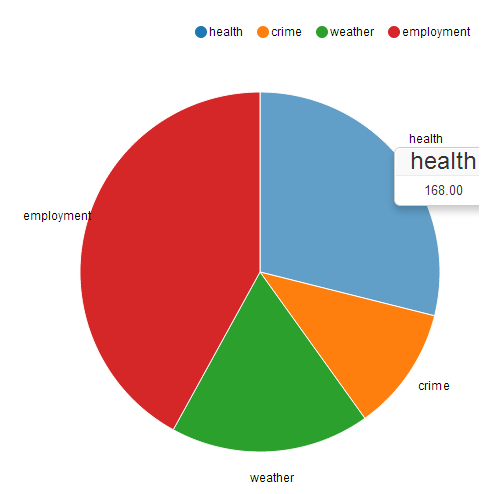
\includegraphics[height=3in, width=3in]{2.png}
\label{2}
\end{figure}

\subsection{Map-annotation}
\textit{Input}  Input to ‘Map-annotation’ module is the latitudes and longitudes of the place entered. 

\textit{Service required} We used ‘Google-maps’ API to get the coordinates of the place entered. As a user enters a name of a place as a string, ‘Google-maps’ is called to return the corresponding coordinates to the location entered. Those coordinates are then passed to ‘Leaflet’ javascript library to generate the map annotation. 

\textit{Result} Result is an annotated map showing the location entered.


\begin{figure}[h]
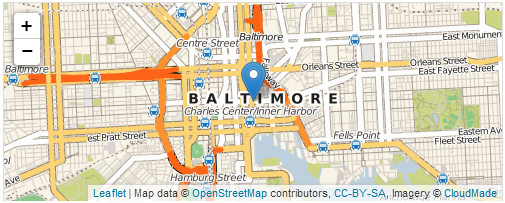
\includegraphics[height=2in, width=2.5in]{3.png}
\label{3}
\end{figure}

\subsection{Tag-cloud}

\textit{Input}  Input to ‘tag-cloud’ module is a list of keywords associated with the categories.

\textit{Service required}  We used REST to pass the JSON object from python API Flask to the ‘d3’ Javascript library. JSON object is then read level by level to get the keywords under each category for the queried place. A data structure having all the keywords is then passed to ‘tag-cloud’ Javascript library. 

\textit{Result}  A tag-cloud having all the keywords is then presented on the analysis page. 

\begin{figure}[h]

\includegraphics[height=2in, width=2.5in]{4.png}
\label{3}
\end{figure}

\subsection{Comparison}

\textit{Input} Input to comparison module is a pair of data structures containing the frequency of keywords corresponding to a category for two different locations. 

\textit{Service required} JSON objects are first created using the data retrieved from database corresponding to the places. JSON objects are then read level by level to get the frequency of keywords corresponding to each category. Data structures are created are then created and passed to pie chart module to create two different pie charts. 

\textit{Results} Two different pie charts are shown on the analysis page comparing the trends in two locations entered. 

\begin{figure}[h]
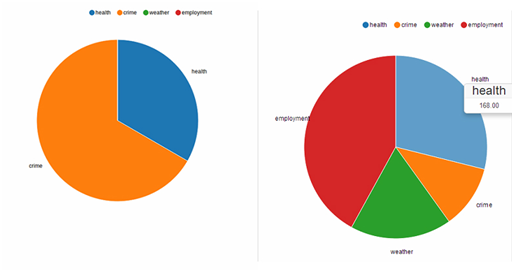
\includegraphics[height=2in, width=3in]{5.png}
\label{5}
\end{figure}

\section{Data}

\subsection{Big Data Source}

a)  Based on the goals of the project, the original data source needed to be all the web pages on the Internet. As opposed to going through and collecting all the web pages into a local storage site, Amazon Web Service’s (AWS) common crawl data was used \cite{amazon:aws}. Amazon’s common crawl is a web crawl of billions of web pages. The data is free and open source, allowing us to access all the data necessary to provide the user with useful information. The data came in 2 different formats, the ARC file and plain old text files. The ARC files are full HTTP responses, containing HTTP headers and content. The other format option is text files in UTF-8 format. Text files are claimed to be 20\% smaller than the ARC files as they are simply the raw web pages, not full HTTP responses \cite{commoncrawl:data}. For the purposes of Centipede, since textual analysis on the web pages will be done, text files were used to perform the necessary analysis. 

\subsection{Database Storage}
a)  Once the data was collected from the AWS, the data needed to be processed and stored in a database for easy retrieval from the user interface. The raw text files were put through MapReduce jobs on Hadoop machines in order to extract the necessary information, and then store it in the database. The description for each step in the data processing and viewing is provided in the Technologies and Hardware section. Once the data has been processed, it is stored in a local MongoDB database in a specific Javascript Object Notation (JSON) format. The general format for the JSON is shown below.

\begingroup
    \fontsize{8pt}{10pt}
\begin{verbatim} 

{
“_id”:”location” 
“location”: 
{ 
    “category1”:
    {
      “keyword1”: 
        {
          “data”: 
          { 
            information from Alchemy API, 
            “metadata”: 
            { 
              author, title, etc from the article
      }}
    }
  }
}

\end{verbatim}
\endgroup

The JSON structure stored in the database. Note that the Information from Alchemy API is listed, but not specified as it is specified in the Technologies and Hardware section. 

The user interface then retrieves and displays the information found in the most nested level of the JSON. 


\section{Technologies \& Hardware}

\subsection{Onelook dictionary}

a)  The OneLook Reverse Dictionary allows us to type in a context, and then it will provide a list of keywords that are associated with that context \cite{beeferman:onelook}. This gave us the chance to enter in our contexts, which are health, crime, employment, and weather, and retrieve a large list of keywords that are commonly associated with that context. Using this as a reference, the article was scanned in mapper and any word that came up in our dictionary was then stored and passed in to the reducer.

\subsection{Alchemyapi}

a)  Alchemy API is an online API that performs Natural Language Processing (NLP) on any given input text. It extracts entites, keywords, etc from the provided input \cite{alchemyapi:alchemy}. Alchemy API provides all the tools we need, and all the computation necessary for the purposes of centipede. The primary limitation for Alchemy API was the restriction to send out only 1000 API calls per day with the free registration. 

\subsection{MongoDB}

MongoDB is an open source, NoSQL based database written in C++ \cite{mongo:mongodb}. The reason a NoSQL approach was chosen as opposed to standard SQL is due to the rigidity of the relational table structure. In a relational table, fields and values must be properly defined (columns must not be null, primary keys established, etc). On the other hand, the NoSQL approach gives us the flexibility to use JSON objects, meaning we can define as many fields as we want at any point in time. The JSON objects allows us to create nested structures that can be easily iterated over, and manipulated. Queries are also simple, and intuitive for programmers. There is no need to learn SQL if it is not known. The flexibility of MongoDB made it a better choice than standard SQL for the purposes of Centipede

\subsection{Javascript libraries}

a)  The UI was implemented using standard HTML and several Javascript (JS) libraries. These JS libraries were d3, leaflet, and tagcloud. The d3 library is a data visualization library written in JS \cite{bostock:dthree}. This library was used to create any charts for the UI. The leaflet library is a JS library that creates mobile friendly, interactive maps \cite{agafonkin:leaflet}. This allows us to put a map of the location the user provides to the UI, giving them an idea of what location they just selected. The final library used was the tagcloud library. A tagcloud is simply a group of words of different sizes organized in the shape of a cloud \cite{groves:tagcloud}. The tagcloud library allowed us to create a simple tagcloud, sizing the words based on their relevance to the location. 

\section{Software Architecture}

\subsection{Hadoop and Mapreduce}

\subsubsection{Mapper}

The algorithm for the MapReduce portion is presented below \\

\textit{procedure mapper} \\ 
\textit{inputs}: text file, type: raw AWS text file \\
\textit{outputs}: list of entities from AlchemyAPI, type: List  \\
\textit{Steps} \\
\begin{enumerate}     
\item  Convert text file to a String 
\item Identify the article contents for the text file 
\item Call Alchemy web API sending article contents as input 
\item Add the JSON to the list of entities from AlchemyAPI
\item Go through the article and save any words that are not common English language words. These English language words were taken from the OneLook Reverse Dictionary and saved in a Map in the program 
\item Repeat steps 1 - 4 for the remaining text files
\item Return received Alchemy API output
\item END
\end{enumerate}       

\subsubsection{Reducer}

The steps for the mapper are simple and easy to follow. The mapper is run across all the articles downloaded from the AWS. One major difficulty faced was that only 1,000 articles were downloaded at a time from AWS due to the limitation of local hard disk space, limiting the ability to process more data quickly. Locations were also defined by the google maps API to confirm whether the location is in fact a valid location, and not just any entity. 

The reducer simply took the JSON from before, and converted it to the JSON format from Figure 1, and then stored the newly formatted JSON in the database. The algorithm is presented below

\textit{procedure reducer} \\
\textit{inputs:} list of entities from AlchemyAPI, type: List  \\
\textit{outputs}: none (JSON stored directly in database) \\
\textit{Steps} \\
\begin{enumerate} 
\item Create HashMap String, List Information organized by context
\item Take entities and their associated data in the JSON from the mapper and store them in a HashMap by parsing through the JSON. \\ \indent Note, the only required information is relevance, frequency, and overall sentiment for the keyword. These values are stored in the List for the HashMap
\item If the entity is already exists in the HashMap add the Alchemy API information to the currently growing list 
\item If the list already contains the given keyword and context, average out the frequency and relevance, and pick the appropriate sentiment 
\item The sentiment is chosen by picking the comparing it to the current sentiment stored, and seeing if the relevance of the new sentiment is greater or less then the relevance of the old sentiment. The sentiment with the higher relevance to the entity based on Alchemy API will be stored in the HashMap 
\item Once all the entities have been processed, iterate over the map, create a JSON object out of each key, value pair in the HashMap. \\ \indent The JSON object is created using a toString() method called for each key, value pair. The output of the toString() is then stored in a local string variable 
\item The local string is written to a file called MongoDB.json on the local hard disk. Refer to Figure 1 for the JSON structure 
\item Each entity is appended to the end of the local file 
\end{enumerate}

After the reducer finishes writing the JSON to the json file, the file is the manually imported into MongoDB using a simple command to store all the JSON objects in the file. In order to assign each word to a specific context, a python program was written to take the output from the OneLook Reverse Dictionary. The reducer function then organized the keywords accordingly based on our OneLook Reverse Dictionary 

\subsection{REST API}

The REST API used for communication between the database and the UI was written in Python using the Flask framework. Flask is a micro webdevelopment framework for Python, that allows us to develop the REST API for sending and receiving data from the database to the UI \cite{ronacher:flask}. 


\subsection{Project Architecture}

\begin{figure}[h]
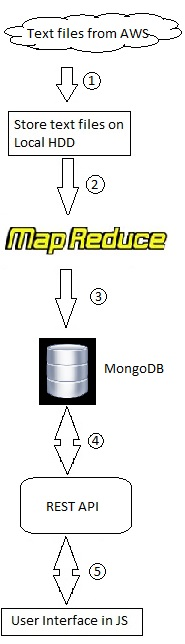
\includegraphics[height=2.5in, width=1.7in]{software_architecture.jpg}
\caption{Project Architecture Diagram}
\label{archi}
\end{figure}

The diagram above shows the data flow for the entire process. (1) is simply downloading the raw text files from the AWS to the local hard drive to make for easier processing. (2) inputs the raw text files to the Hadoop MapReduce jobs. (3) takes the output from the reducer and stores it in the database in the JSON format from Figure 1. (4) is when the REST API contacts the Database and retrieves any information that the UI requests. (5) the UI sends the request to the REST API, asking for the specific entity/location and get the JSON object associated with that entity. 

\section{Evaluation}

We evaluated centipede by comparing the words retrieved by our system with the important keywords extracted from Wikipedia. Python libraries like BeautifulSoup and Topia.TermExtract were used for processing html and extracting keywords from webpage respectively \cite{scrap:it}.  The keywords extracted from Wikipedia were considered as the relevant keywords and centipede results were considered as retrieved keywords. We calculated precision, recall and F1 score using these two results.


The following table summarizes the results of evaluation for the location search of the four locations; Baltimore, Omaha and Cleveland.

\begin{figure}[h]
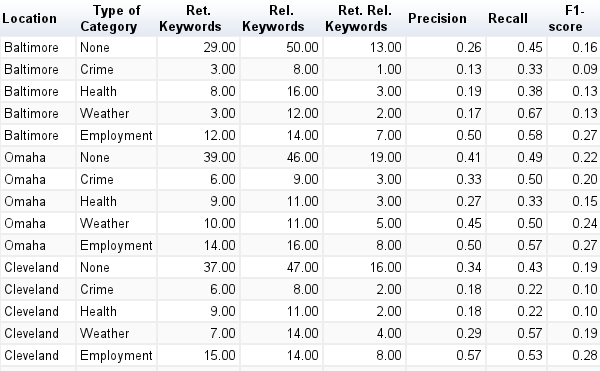
\includegraphics[height=3in, width=3in]{table_sample.png}
\caption{Evaluation results}
\label{table}
\end{figure}

The precision metric finds the proportion of relevant keywords from the results.
\begin{equation}
precision (per \hspace{1mm} category) = \frac{\text{retrieved keywords} \cap \text{relevant keywords}} {\text{retrieved keywords}}
\end{equation}

\begin{figure}[h]
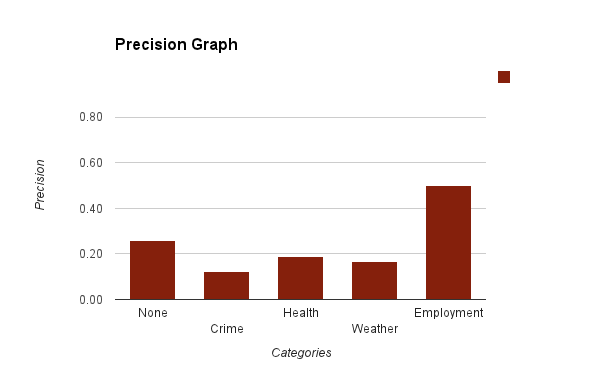
\includegraphics[height=3in, width=4in]{precision.png}
\caption{Precision measures for various categories of Baltimore}
\label{precision}
\end{figure}

The recall measures the ratio of retrieved keywords which are relevant against relevant keywords.
\begin{equation}
recall (per \hspace{1mm} category) = \frac{\text{retrieved keywords} \cap \text{relevant keywords}} {\text{relevant keywords}}
\end{equation}

\begin{figure}[h]
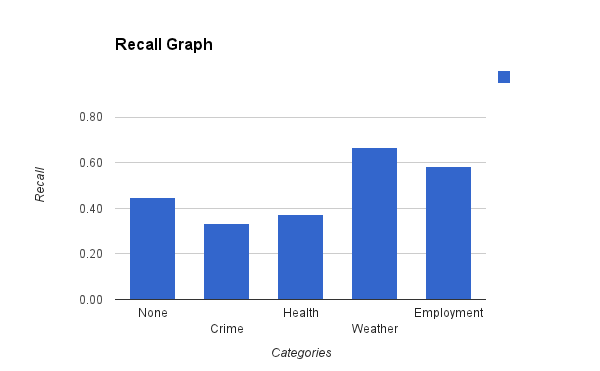
\includegraphics[height=3in, width=4in]{recall.png}
\caption{Recall measures for various categories of Baltimore}
\label{recall}
\end{figure}

The F1 score is another metric to evaluate accuracy.  It considers both precision and recall measures of a test to compute the score. In information retrieval systems, it is considered a single value obtained combining both the precision and recall measures and indicates an overall utility of result.\footnote{http://aimotion.blogspot.com/2011/05/evaluating-recommender-systems.html}
\begin{equation}
F1 score = 2 * \frac{precision * recall}{precision + recall}
\end{equation}

\begin{figure}[h]
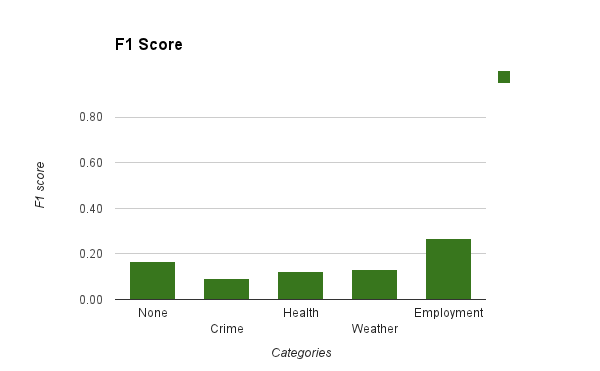
\includegraphics[height=3in, width=4in]{f1score.png}
\caption{F1-score for various categories of Baltimore}
\label{f1}
\end{figure}


\section{Challenges}

We had to face two major kinds of challenges while developing Centipede: Handling the huge web crawl data corpus and big data analysis interpretation. As of today, the web corpus is over 81 TB and we could process a small portion of this data. Being Open Source, it was fairly straightforward to get access to the data. After getting access to data, we found out that it was stored in a distributed manner on Amazon Web Services across a number of buckets\cite{aws:bucket}. As the crawl is ongoing, the data had a mixture of valid and invalid segments. Luckily we came across a blog post which mentions the valid segments and we used it to download the valid segments. Initially we downloaded to local hard disk and then manually moved it to HDFS, but we quickly ran out of space due to this redudancy. So we decided to download it straight to HDFS.

The second challenge was that of analyzing this large dataset. We had to clean up the noise; metadata, http requests, response and multiple languages from the data before feeding it to mapreduce. We used the streaming library of Hadoop and used Java and Python to code Mapreduce jobs. This saved us significant amount of development time but at the cost of processing time. Similarly, although Alchemy API made our life easier for analyzing the data, it had significant limitations in terms of number of requests per day and concurrent requests.

We also had to overcome other challenges in project integration and system administration during the course of the project. Our previous experience with Github for version control and Amazon Web Services for deployment made these aforementioned tasks easier. 

\section{Future work}

The excitement about Open Source web crawl data motivated us to develop centipede. When we were in the final stages of our project, a newer version of web crawl data was released and we were not able to use it in our project. In a future version of the project, we would like to implement an infrastructure which would dynamically update the database whenever newer releases of Commoncrawl are released. For this, we will need to move our hadoop infrastructure to either Bluegrit or Amazon Web services Elastic Mapreduce \cite{aws:emr}. 

We did single word analysis for learning about context of a location. We believe a bi-gram or n-gram analysis could improve the value of information generated by the system. By relying on entity reasoning and disambiguation, we would be able to improve the precision of Centipede.   

The results from evaluating Centipede shows that web crawl data can be an important source for learning about a location. Additionally we could build recommender systems and other context-aware systems on top of this to leverage results from centipede. In terms of evaluation, it will be interesting to see how would the results from centipede compare against other sources of information like Internet news.

\section{Student roles}

We divided the project responsibilites into three: Big data analysis, REST API and user Interface; with each of the team member responsible for one of the three parts. Primal worked on setting up the Hadoop cluster and experimenting with various streaming apis. He also helped Abhishek in developing the Mapreduce algorithm. He also developed the reverse dictionary and the REST API using python. Abhishek used Alchemyapi to analyze the web crawl data and stored results in JSON format in Mongodb. He also cleaned up the data and worked closely with Vikas to finalize the data representation format. Vikas worked on the user interface. He created the home page of our service using twitter bootstrap. Using javascript libraries such D3 and LeafLet he visualized the results provided by REST API from Mongodb. He generated WSDL code for the service. We worked together on the proposal, midterm and final presentations as well as the final project report. 

\section*{Acknowledgment}

We would like to thank the reviewers for evaluating our project through all the stages and giving very valuable feedback. A special thanks to Dr. Halem, his Teaching Assistant, Lawrence Sebald for their patience in guiding us through the project.  

% trigger a \newpage just before the given reference
% number - used to balance the columns on the last page
% adjust value as needed - may need to be readjusted if
% the document is modified later
%\IEEEtriggeratref{8}
% The "triggered" command can be changed if desired:
%\IEEEtriggercmd{\enlargethispage{-5in}}

% references section

% can use a bibliography generated by BibTeX as a .bbl file
% BibTeX documentation can be easily obtained at:
% http://www.ctan.org/tex-archive/biblio/bibtex/contrib/doc/
% The IEEEtran BibTeX style support page is at:
% http://www.michaelshell.org/tex/ieeetran/bibtex/
%\bibliographystyle{IEEEtran}
% argument is your BibTeX string definitions and bibliography database(s)
%\bibliography{IEEEabrv,../bib/paper}
%
% <OR> manually copy in the resultant .bbl file
% set second argument of \begin to the number of references
% (used to reserve space for the reference number labels box)
\begin{thebibliography}{1}

\bibitem{semsim:lushan}
Han, Lushan, Tim Finin, and Anupam Joshi. \emph{Schema-free structured querying of dbpedia data} Proceedings of the 21st ACM international conference on Information and knowledge management. ACM, 2012.

\bibitem{pr:page}
Page, Lawrence and Brin, Sergey and Motwani, Rajeev and Winograd, Terry. \emph{The PageRank Citation Ranking: Bringing Order to the Web} Technical Report. Stanford InfoLab, 1999.

\bibitem{db:klu}
Klusch, Matthias, and Patrick Kapahnke. \emph{Web Semantics: Science, Services and Agents on the World Wide Web.} Web Semantics: Science, Services and Agents on the World Wide Web 15 (2012): 1-14.

\bibitem{mo:sens}
Gellersen, Hans W., Albercht Schmidt, and Michael Beigl. \emph{Multi-sensor context-awareness in mobile devices and smart artifacts.} Mobile Networks and Applications 7.5 (2002): 341-351.

\bibitem{abo:wd}
Abowd, Gregory D., et al. \emph{Towards a better understanding of context and context-awareness.} Handheld and ubiquitous computing. Springer Berlin Heidelberg, 1999.

\bibitem{med:one}
DellaVigna, Stefano, and Ethan Kaplan. \emph{The Fox News effect: Media bias and voting.} The Quarterly Journal of Economics 122.3 (2007): 1187-1234.

\bibitem{med:two}
Groseclose, Tim, and Jeffrey Milyo. \emph{A measure of media bias.} The Quarterly Journal of Economics 120.4 (2005): 1191-1237.


\bibitem{scrap:it}
\emph{http://scrapit.herokuapp.com/} 

\bibitem{aws:bucket}
\emph{http://aws.amazon.com/s3/}

\bibitem{aws:emr}
\emph{http://aws.amazon.com/elasticmapreduce/}

\bibitem{ronacher:flask}
Ronacher, Armin. \emph{Welcome to Flask} http://flask.pocoo.org/docs/

\bibitem{groves:tagcloud}
Groves, Adam. \emph{jquery.tagcloud.js}.https://github.com/addywaddy/jquery.tagcloud.js/

\bibitem{agafonkin:leaflet}
Agafonkin, Vladmir. \emph{Leaflet} http://leafletjs.com/\#getting-involved

\bibitem{bostock:dthree}
Bostock, Mike. \emph{D3 Data-Driven Documents} http://d3js.org/

\bibitem{beeferman:onelook}
Beeferman, Doug. \emph{OneLook Reverse Dictionary} http://www.onelook.com/reverse-dictionary.shtml

\bibitem{alchemyapi:alchemy}
\emph{Alchemy API} http://www.alchemyapi.com/

\bibitem{mongo:mongodb}
\emph{mongoDB} http://www.mongodb.org/

\bibitem{amazon:aws}
\emph{Amazon Web Services} http://aws.amazon.com/

\bibitem{commoncrawl:data}
\emph{Data|Common Crawl} commoncrawl.org/data/


\end{thebibliography}

\pagebreak

\onecolumn

\section{Appendix}


\subsection{WSDL}

\begin{verbatim}

<?xml version="1.0" encoding="UTF-8"?>
<wsdl:definitions targetNamespace="http://centipede.com" xmlns:apachesoap="http://xml.apache.org/xml-soap" xmlns:impl="http://centipede.com" xmlns:intf="http://centipede.com" xmlns:wsdl="http://schemas.xmlsoap.org/wsdl/" xmlns:wsdlsoap="http://schemas.xmlsoap.org/wsdl/soap/" xmlns:xsd="http://www.w3.org/2001/XMLSchema">
<!--WSDL created by Apache Axis version: 1.4
Built on Apr 22, 2006 (06:55:48 PDT)-->
 <wsdl:types>
  <schema elementFormDefault="qualified" targetNamespace="http://centipede.com" xmlns="http://www.w3.org/2001/XMLSchema">
   <element name="getPrefix">
    <complexType>
     <sequence>
      <element name="_prefix" type="xsd:string"/>
     </sequence>
    </complexType>
   </element>
   <element name="getPrefix2">
    <complexType>
     <sequence>
      <element name="_prefix2" type="xsd:string"/>
     </sequence>
    </complexType>
   </element>
   <element name="getPrefixResponse">
    <complexType>
     <sequence>
      <element name="getPrefixReturn" type="xsd:string"/>
     </sequence>
    </complexType>
   </element>
  </schema>
 </wsdl:types>

   <wsdl:message name="getPrefixResponse">

      <wsdl:part element="impl:getPrefixResponse" name="parameters">

      </wsdl:part>

   </wsdl:message>

   <wsdl:message name="getPrefixRequest">

      <wsdl:part element="impl:getPrefix" name="parameters">

      </wsdl:part>

   </wsdl:message>

   <wsdl:portType name="Getplace">

      <wsdl:operation name="getPrefix">

         <wsdl:input message="impl:getPrefixRequest" name="getPrefixRequest">

       </wsdl:input>

         <wsdl:output message="impl:getPrefixResponse" name="getPrefixResponse">

       </wsdl:output>

      </wsdl:operation>

   </wsdl:portType>

   <wsdl:binding name="GetplaceSoapBinding" type="impl:Getplace">

      <wsdlsoap:binding style="document" transport="http://schemas.xmlsoap.org/soap/http"/>

      <wsdl:operation name="getPrefix">

         <wsdlsoap:operation soapAction=""/>

         <wsdl:input name="getPrefixRequest">

            <wsdlsoap:body use="literal"/>

         </wsdl:input>

         <wsdl:output name="getPrefixResponse">

            <wsdlsoap:body use="literal"/>

         </wsdl:output>

      </wsdl:operation>

   </wsdl:binding>

   <wsdl:service name="GetplaceService">

      <wsdl:port binding="impl:GetplaceSoapBinding" name="Getplace">

         <wsdlsoap:address location="http://localhost:8080/Centipede/services/Getplace"/>

      </wsdl:port>

   </wsdl:service>

</wsdl:definitions>

<?xml version="1.0" encoding="UTF-8"?>
<wsdl:definitions targetNamespace="http://centipede.com" xmlns:apachesoap="http://xml.apache.org/xml-soap" xmlns:impl="http://centipede.com" xmlns:intf="http://centipede.com" xmlns:wsdl="http://schemas.xmlsoap.org/wsdl/" xmlns:wsdlsoap="http://schemas.xmlsoap.org/wsdl/soap/" xmlns:xsd="http://www.w3.org/2001/XMLSchema">
<!--WSDL created by Apache Axis version: 1.4
Built on Apr 22, 2006 (06:55:48 PDT)-->
 <wsdl:types>
  <schema elementFormDefault="qualified" targetNamespace="http://centipede.com" xmlns="http://www.w3.org/2001/XMLSchema">
   <element name="getPrefix">
    <complexType>
     <sequence>
      <element name="_prefix" type="xsd:string"/>
     </sequence>
    </complexType>
   </element>
   <element name="getPrefix2">
    <complexType>
     <sequence>
      <element name="_prefix2" type="xsd:string"/>
     </sequence>
    </complexType>
   </element>
   <element name="getPrefixResponse">
    <complexType>
     <sequence>
      <element name="getPrefixReturn" type="xsd:string"/>
     </sequence>
    </complexType>
   </element>
  </schema>
 </wsdl:types>

   <wsdl:message name="getPrefixResponse">

      <wsdl:part element="impl:getPrefixResponse" name="parameters">

      </wsdl:part>

   </wsdl:message>

   <wsdl:message name="getPrefixRequest">

      <wsdl:part element="impl:getPrefix" name="parameters">

      </wsdl:part>

   </wsdl:message>

   <wsdl:portType name="Getplace">

      <wsdl:operation name="getPrefix">

         <wsdl:input message="impl:getPrefixRequest" name="getPrefixRequest">

       </wsdl:input>

         <wsdl:output message="impl:getPrefixResponse" name="getPrefixResponse">

       </wsdl:output>

      </wsdl:operation>

   </wsdl:portType>

   <wsdl:binding name="GetplaceSoapBinding" type="impl:Getplace">

      <wsdlsoap:binding style="document" transport="http://schemas.xmlsoap.org/soap/http"/>

      <wsdl:operation name="getPrefix">

         <wsdlsoap:operation soapAction=""/>

         <wsdl:input name="getPrefixRequest">

            <wsdlsoap:body use="literal"/>

         </wsdl:input>

         <wsdl:output name="getPrefixResponse">

            <wsdlsoap:body use="literal"/>

         </wsdl:output>

      </wsdl:operation>

   </wsdl:binding>

   <wsdl:service name="GetplaceService">

      <wsdl:port binding="impl:GetplaceSoapBinding" name="Getplace">

         <wsdlsoap:address location="http://localhost:8080/Centipede/services/Getplace"/>

      </wsdl:port>

   </wsdl:service>

</wsdl:definitions>



\end{verbatim}

\subsection{REST API}

\subsubsection{Request}

\begin{verbatim}

http://ec2-54-197-119-222.compute-1.amazonaws.com/locationsearch?location1=omaha&location2=chicago
\end{verbatim}

\begin{itemize}
\item location1 contains the string representing the location name of one of the cities. 
\item location2 contains the name of the other city with which we want to compare the first location. 
\end{itemize}
Response to this request is a webpage having analysis of the data corresponding to both the cities. Response codes are generated with the response to a particular request. Following are some codes implemented in our service

\begin{itemize}
\item 200 OK: This response code indicates that the request was successful.
\item 400 Bad Request: The request was malformed. This happens especially with POST and PUT requests, when the data does not pass validation, or is in the wrong format
\item 404 Not Found: This response indicates that the required resource could not be found. This is generally returned to all requests which point to a URL with no corresponding resource.
\end{itemize}

\subsubsection{Response}

JSON object is returned in the response by the REST API.
\begin{verbatim}
{ "_id": "Baltimore, MD",
    "category": {
    "health": {
      "hospital": {
        "data": {"frequency": 3, "relevance": 0.7845, "sentiment": "Mixed"},
        "metadata": {
          "article1": {"author": "Tom Jones", "title": "Current Rises in Health Insurance Policies in Baltimore", "timestamp": "26-FEB-1987 15:01:01.79"},
          "article2": {"author": "Bob Jenkins", "title": "Obamacare in Hospitals", "timestamp": "06-SEP-2011 16:32:34.73"},
          "article3": {"author": "Tom Jones", "title": "Rises in Hospital Fees", "timestamp": "31-DEC-1991 01:45:59.66"}
        } 
      } 
    },
    "crime": {
      "assault": {
        "data": {"frequency": 12, "relevance": 0.9045, "sentiment": "Negative"},
        "metadata": {
          "article1": {"author": "", "title": "Another shooting in Baltimore", "timestamp": "26-FEB-1987 15:01:01.79"},
          "article2": {"author": "Anderson Silva", "title": "Street Crime up in cities", "timestamp": "06-SEP-2011 16:32:34.73"},
          "article3": {"author": "John Jones", "title": "Rise in assaults in Baltimore", "timestamp": "31-DEC-1991 01:45:59.66"}
        } 
      },
      "robbery": {
        "data": {"frequency": 15, "relevance": 0.553, "sentiment": "Positive"},
        "metadata": {
          "article1": {"author": "Rob", "title": "Robbery of Museum in Baltimore", "timestamp": "26-FEB-1987 15:01:01.79"},
          "article2": {"author": "Anderson Silva", "title": "Man held at gunpoint for wallet", "timestamp": "06-SEP-2011 16:32:34.73"},
          "article3": {"author": "John Jenkins", "title": "Increase in robbery frequency in MD", "timestamp": "31-DEC-1991 01:45:59.66"}
        } 
      }       
    }
  }
}

{ "_id": "Germantown, MD",
  "category": {
    "health": {
      "hospital": {
        "data": {"frequency": 23, "relevance": 0.7845, "sentiment": "Positive"},
        "metadata": {
          "article1": {"author": "Tom Jones", "title": "Small suburbs affected by rise in healthcare prices", "timestamp": "26-FEB-1987 15:01:01.79"},
          "article2": {"author": "Bob Jenkins", "title": "Newly opened Emergency ROom in Germantown MD", "timestamp": "06-SEP-2011 16:32:34.73"}
        } 
      } 
    },
    "weather": {
      "heat": {
        "data": {"frequency": 22, "relevance": 0.9045, "sentiment": "Negative"},
        "metadata": {
          "article1": {"author": "", "title": "Heat wave scorches the east coast", "timestamp": "26-FEB-1987 15:01:01.79"}
        } 
      },
      "snow": {
        "data": {"frequency": 15, "relevance": 0.553, "sentiment": "Positive"},
        "metadata": {
          "article1": {"author": "Rob", "title": "Large snow storm to hit East Coast", "timestamp": "26-FEB-1987 15:01:01.79"},
          "article2": {"author": "Ron Wesley", "title": "Snow from west heading towards the Bay area", "timestamp": "26-FEB-1987 15:01:01.79"}
        } 
      }       
    }
  }
}
\end{verbatim}


% that's all folks
\end{document}


